\documentclass[tikz,border=10pt]{standalone}
\usetikzlibrary{calc}
\begin{document}
% Pixel coordinates, y flipped, 1 px = 0.01 cm
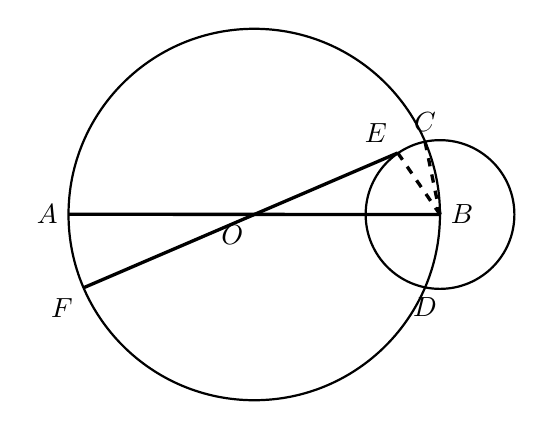
\begin{tikzpicture}[scale=0.01, line join=round, line width=1.2pt]
  % Points (px, y negated)
  \coordinate (O) at (303.5,-264.3);
  \coordinate (A) at (67.4,-264.0);
  \coordinate (B) at (539.7,-264.3);
  % F lies on the large circle (centre O, r=236), on the line E-O extended
  \coordinate (F) at (86.6,-357.4);
  \coordinate (E) at (486.0,-186.0);
  \coordinate (C) at (520.7,-172.0);
  \coordinate (D) at (520.7,-356.6);

  % Circles (thin solid)
  \draw[line width=0.8pt] (O) circle[radius=236.0];
  \draw[line width=0.8pt] (B) circle[radius=94.5];

  % Solid horizontal diameter A-B
  \draw (A) -- (B);

  % Solid straight segment F-O-E
  \draw (F) -- (E);

  % Dashed segments E-B and C-B
  \draw[dashed] (E) -- (B);
  \draw[dashed] (C) -- (B);

  % Labels
  \node[left] at (A) {$A$};
  \node[below left] at (O) {$O$};
  \node[right] at (B) {$B$};
  \node[below left] at (F) {$F$};
  \node[above left] at (E) {$E$};
  \node[above] at (C) {$C$};
  \node[below] at (D) {$D$};
\end{tikzpicture}
\end{document}